\setclass{BubbleAndEat::Restaurant::OrderGateway}
\subsubsection{Server - \class}
\begin{figure}[H]
	\centering
	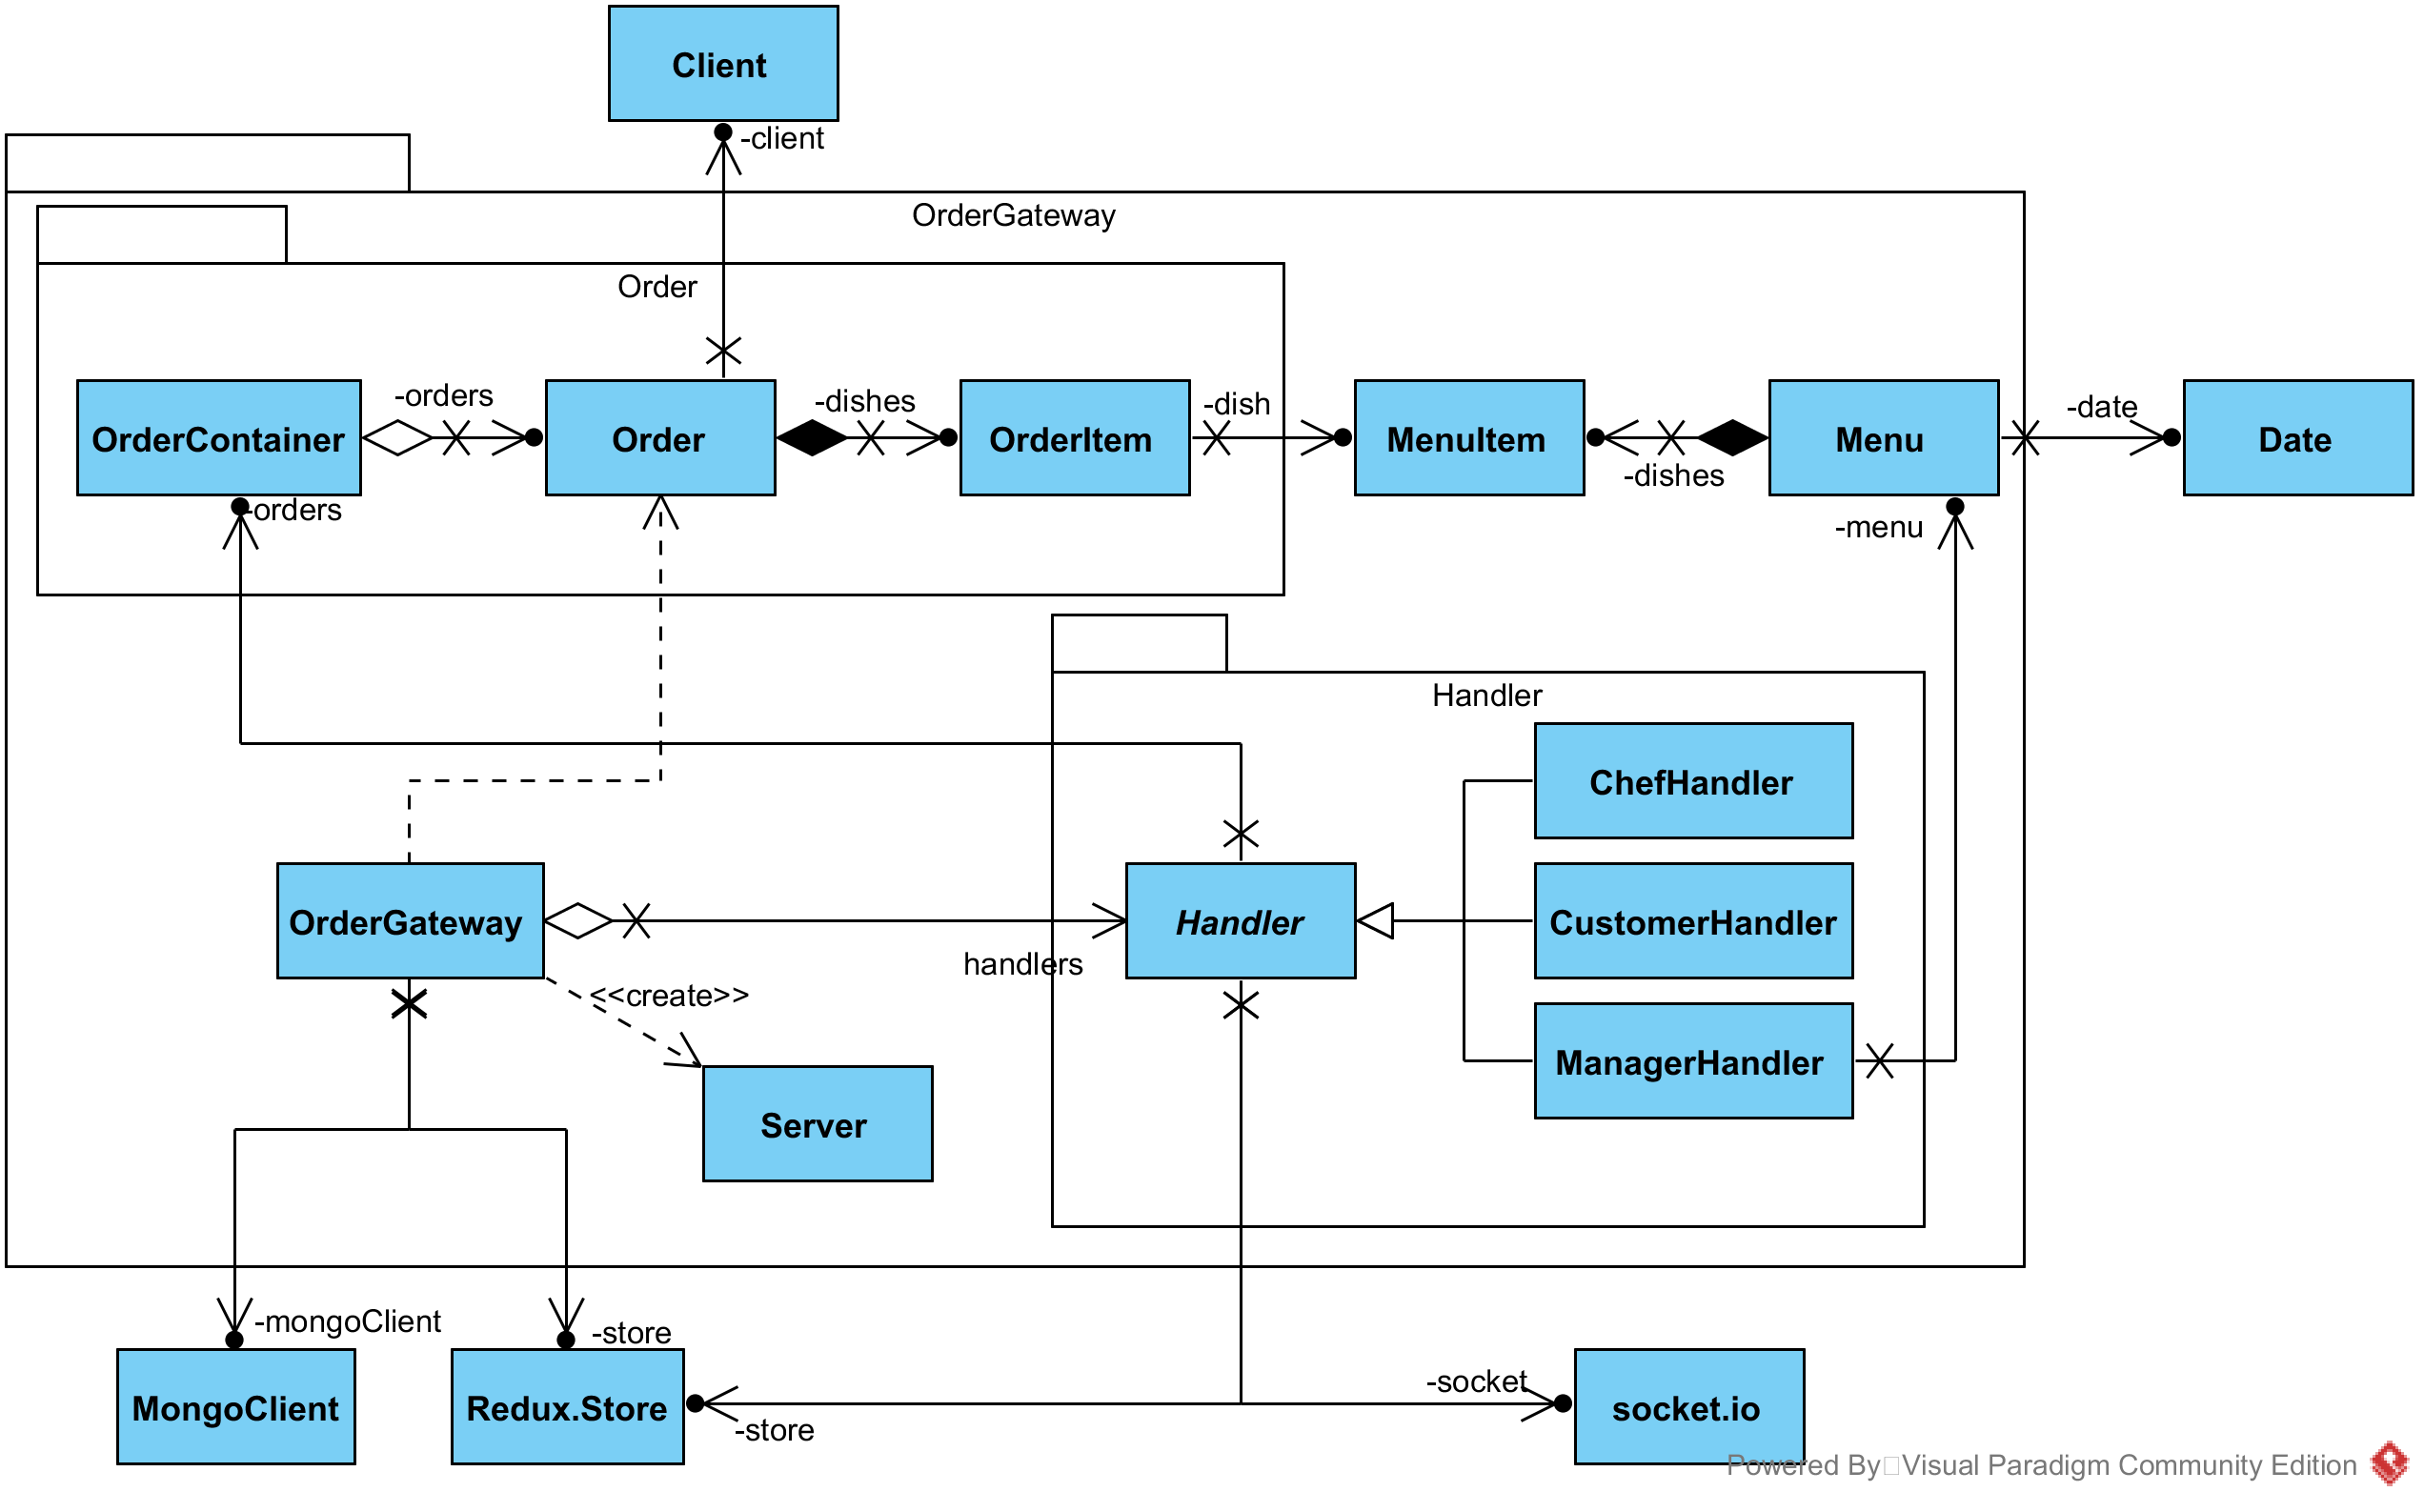
\includegraphics[width=15cm]{./diagrammi/demo/server/ordergatewaypkg.png}
	\caption{Componente \class}
\end{figure}
La parte server della \DemoName{} è formata da OrderGateway, la classe principale che amministra tutte le operazioni legate al server stesso, Server, che crea il server vero e proprio, Menu e MenuItem, che rappresentano il menu del ristorante, e dai package Order e Handler, che si occupano rispettivamente di rappresentare gli ordini e di gestire le richieste da parte delle bubble. 

\setclass{BubbleAndEat::Restaurant::OrderGateway::Server}
\paragraph[::Server]{\class}\mbox{}\\ \label{\class}
\begin{figure}[H]
	\centering
		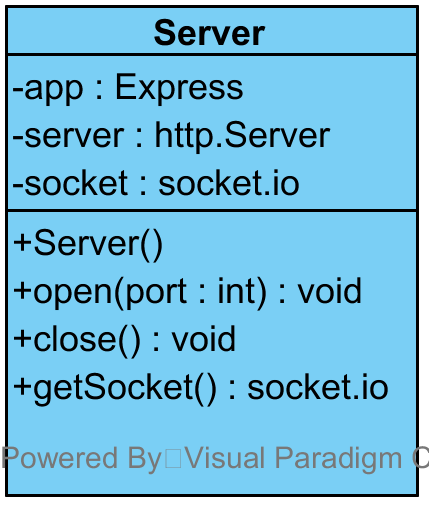
\includegraphics[width=5cm]{./diagrammi/demo/server/server.png}
	\caption{Classe \class}
\end{figure}
\textbf{Descrizione:}\\
Classe che rappresenta il server.

\textbf{Utilizzo:}\\
Viene utilizzata per inizializzare il server stesso e i socket.

%\textbf{Classi ereditate:}
%\begin{itemize}
%	\item \code{}.
%\end{itemize}
%
%\textbf{Sottoclassi:}
%\begin{itemize}
%	\item \coderef{}.
%\end{itemize}

\textbf{Attributi:}
\begin{itemize}
	\item \field{- app: Express}: applicazione Express;
	\item \field{- server: http.Server}: server http;
	\item \field{- socket: socket.io}: socket sul server;
	\item \field{- handlers: Map<string, Handler>}: oggetto che contiene gli handlers associati ad una chiave letterale.
\end{itemize}

\textbf{Metodi:}
\begin{itemize}
	\item \method{+ Server()}: costruttore di default, inizializza gli attributi;
	\item \method{+ open(port: int): void}: mette in ascolto il server sulla porta indicata:
	\begin{itemize}
		\item \param{port: int}: porta da ascoltare;
	\end{itemize}
	\item \method{+ close(): void}: termina il server;
	\item \method{+ getSocket(): socket.io}: getter per \texttt{socket};
\end{itemize}

\setclass{BubbleAndEat::Restaurant::OrderGateway::OrderGateway}
\paragraph[::OrderGateway]{\class}\mbox{}\\ \label{\class}
\begin{figure}[H]
	\centering
	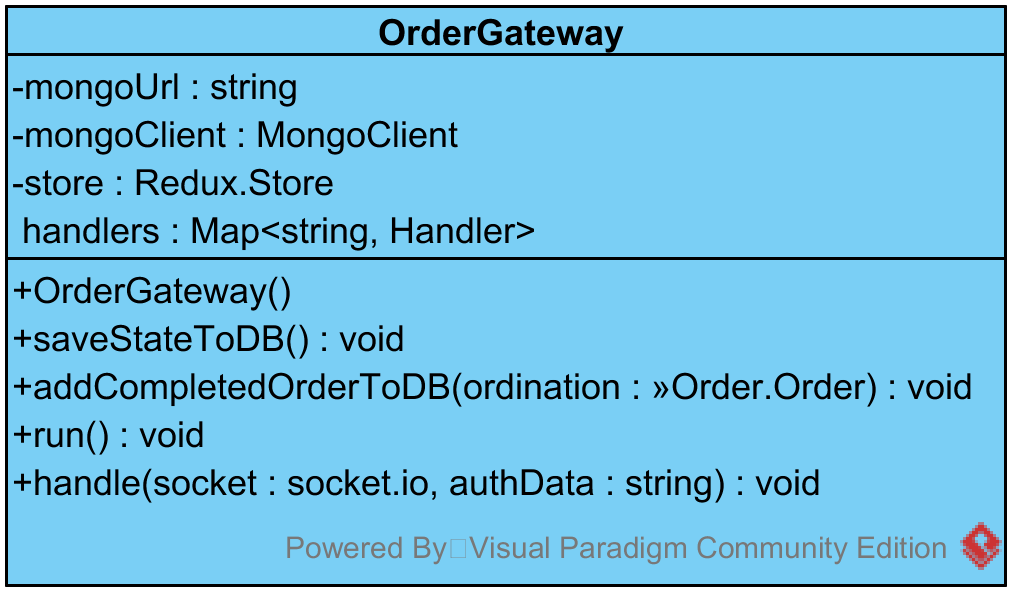
\includegraphics[width=8cm]{./diagrammi/demo/server/ordergateway.png}
	\caption{Classe \class}
\end{figure}
\textbf{Descrizione:}\\
Classe che rappresenta un gateway per le comunicazioni tra le bubble e il server.

\textbf{Utilizzo:}\\
Viene utilizzata per inizializzare le connessioni e indirizzare le comunicazioni alle giuste bubble attraverso appositi handler.

%\textbf{Classi ereditate:}
%\begin{itemize}
%	\item \code{}.
%\end{itemize}
%
%\textbf{Sottoclassi:}
%\begin{itemize}
%	\item \coderef{}.
%\end{itemize}

\textbf{Attributi:}
\begin{itemize}
	\item \field{- mongoClient: MongoClient}: database MongoDB;
	\item \field{- mongoUrl: string}: URI del database;
	\item \field{- store: Redux::Store}: oggetto contenente lo stato dell'applicazione;
	\item \field{- handlers: map<string, Handler>}: oggetto che contiene gli handlers associati ad una chiave letterale.
\end{itemize}

\textbf{Metodi:}
\begin{itemize}
	\item \method{+ OrderGateway()}: costruttore, inizializza lo stato dell'applicazione recuperandolo, se possibile, dal database;
	\item \method{+ saveStateToDB(): void}: effettua la connessione al database e salva lo stato dell'applicazione;
	\item \method{+ addCompletedOrderToDB(ordination: Order): void}: aggiunge l'ordine alla collezione degli ordini completati sul database:
	\begin{itemize}
		\item \param{ordination: Order}: l'ordine completato da aggiungere;
	\end{itemize}
	\item \method{+ run(): void}: avvia il server;
	\item \method{+ handle(socket: socket.io, authData: string): void}: gestisce le connessioni indirizzandole al corretto handler.
\end{itemize}

\setclass{BubbleAndEat::Restaurant::OrderGateway::Handlers}
\paragraph[::Handlers]{\class}\mbox{}\\ \label{\class}
\begin{figure}[H]
	\centering
		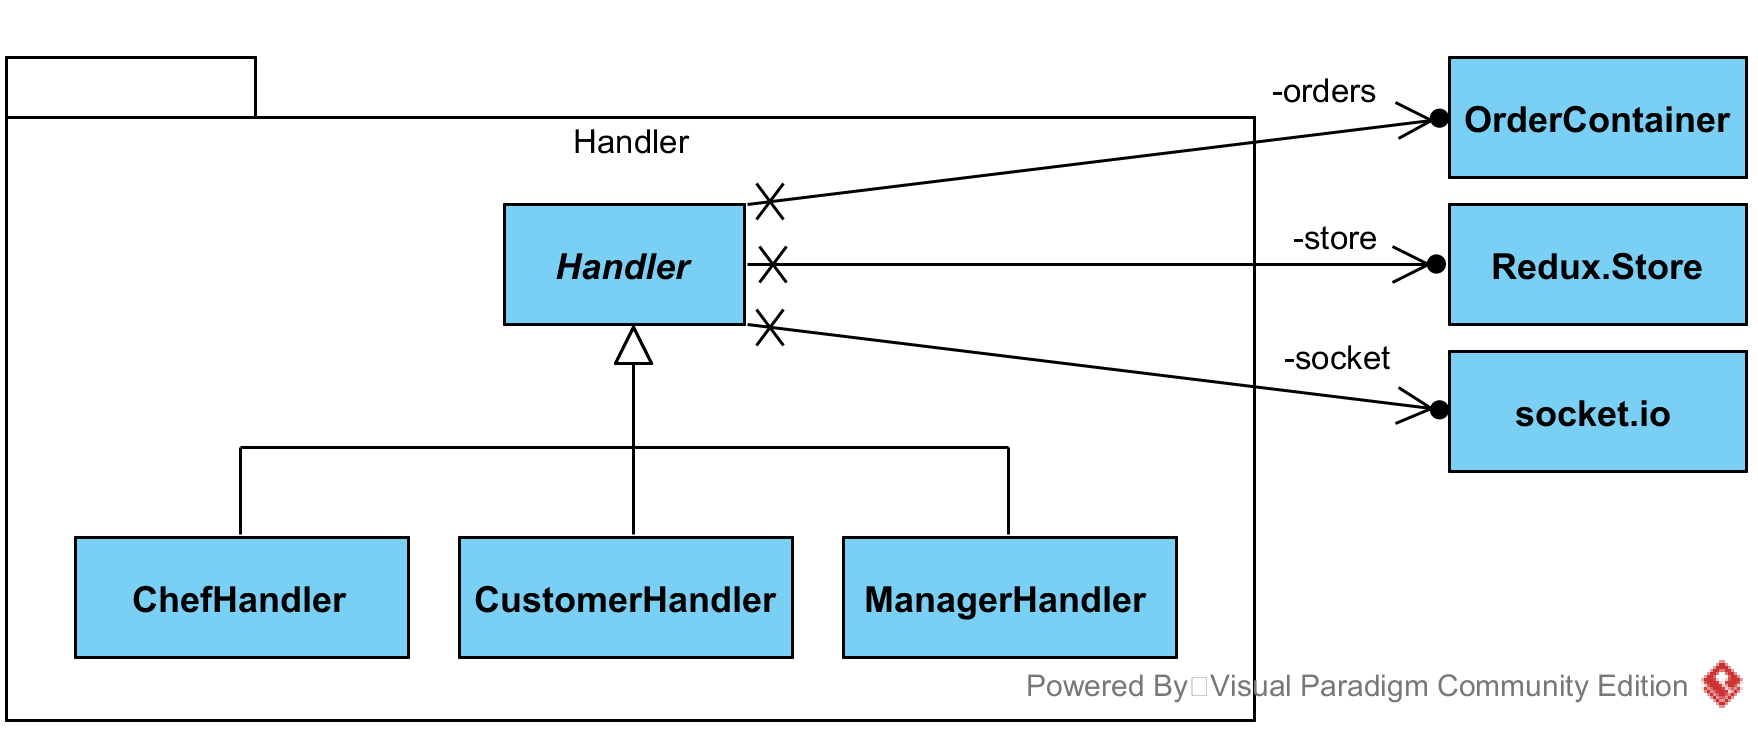
\includegraphics[width=15cm]{./diagrammi/demo/server/handlerpkg.png}
	\caption{Classe \class}
\end{figure}
Questo componente raggruppa gli handler per le varie bubble. Gli handler hanno lo scopo di gestire le richieste delle bubble. Sono presenti ManagerHandler, CustomerHandler e ChefHandler.

\setclass{BubbleAndEat::Restaurant::OrderGateway::Handlers::Handler}
\subparagraph[::Handler]{\class}\mbox{}\\ \label{\class}
\begin{figure}[H]
	\centering
		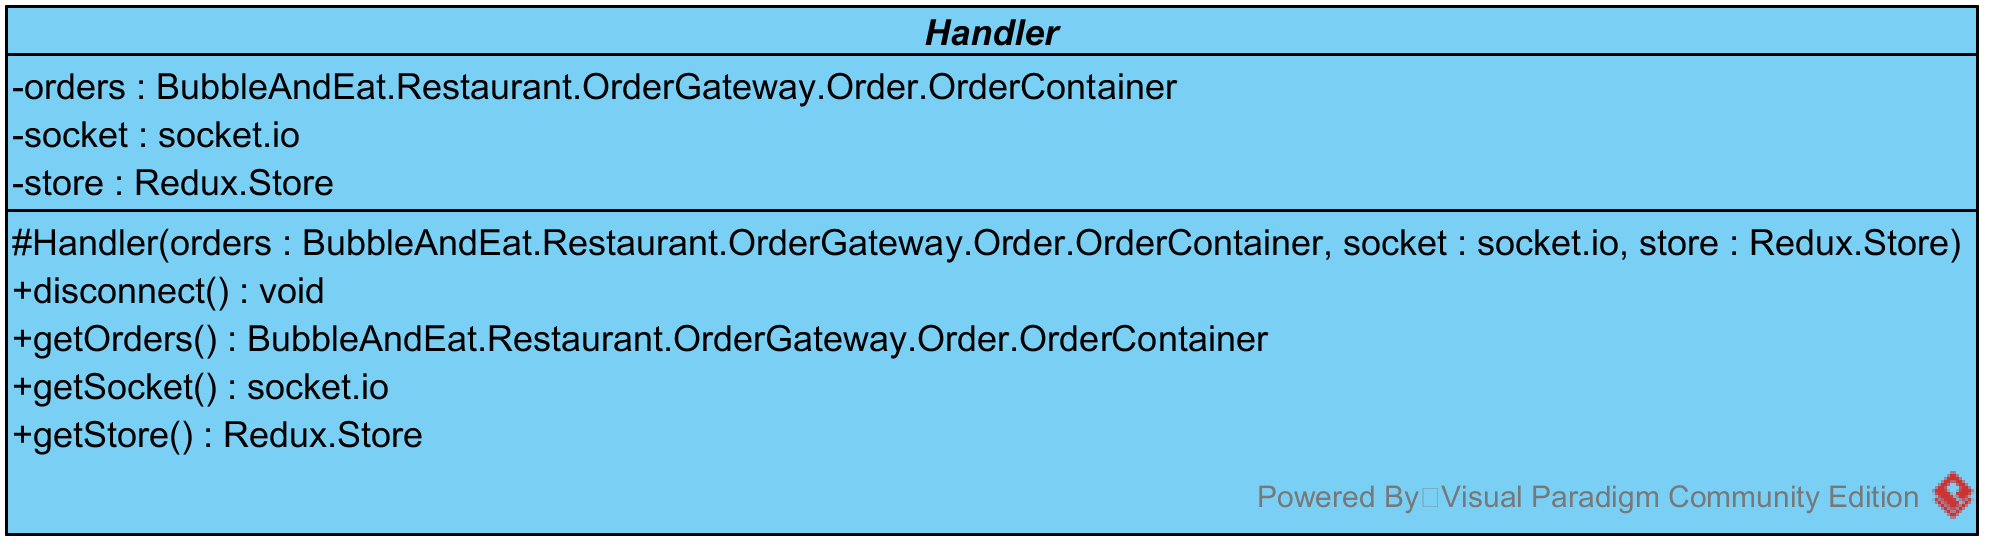
\includegraphics[width=15cm]{./diagrammi/demo/server/handlers/handler.png}
	\caption{Classe \class}
\end{figure}
\textbf{Descrizione:}\\
Classe astratta che fornisce una base comune per gli handlers.

\textbf{Utilizzo:}\\
Viene utilizzata per gestire gli handlers tramite polimorfismo.

%\textbf{Classi ereditate:}
%\begin{itemize}
%	\item \code{}.
%\end{itemize}
%
\textbf{Sottoclassi:}
\begin{itemize}
	\item \coderef{BubbleAndEat::Restaurant::OrderGateway::Handlers::ManagerHandler}.
	\item \coderef{BubbleAndEat::Restaurant::OrderGateway::Handlers::ChefHandler}.
	\item \coderef{BubbleAndEat::Restaurant::OrderGateway::Handlers::CustomerHandler}.
\end{itemize}

\textbf{Attributi:}
\begin{itemize}
	\item \field{- orders: OrderContainer}: ordini del ristorante;
	\item \field{- socket: socket.io}: socket per le comunicazioni con il server;
	\item \field{- store: Redux::Store}: store redux dell'appicazione.
\end{itemize}

\textbf{Metodi:}
\begin{itemize}
	\item \method{\# Handler(orders: OrderContainer[], socket: socket.io, store: Redux::Store)}: costruttore, assegna i parametri agli attributi:
	\begin{itemize}
		\item \param{orders: OrderContainer}: contenitore degli ordini;
		\item \param{socket: socket.io}: socket di connessione;
		\item \param{store: Redux::Store}: store dell'applicazione;
	\end{itemize}
	\item \method{+ getOrders(): OrderContainer}: getter per \texttt{orders};
	\item \method{+ getSocket(): socket.io}: getter per \texttt{socket};
	\item \method{+ getStore(): Redux::Store}: getter per \texttt{store};
	\item \method{+ disconnect(): void}: termina la connessione e le comunicazioni del Manager con il server.
\end{itemize}

\setclass{BubbleAndEat::Restaurant::OrderGateway::Handlers::ManagerHandler}
\subparagraph[::ManagerHandler]{\class}\mbox{}\\ \label{\class}
\begin{figure}[H]
	\centering
		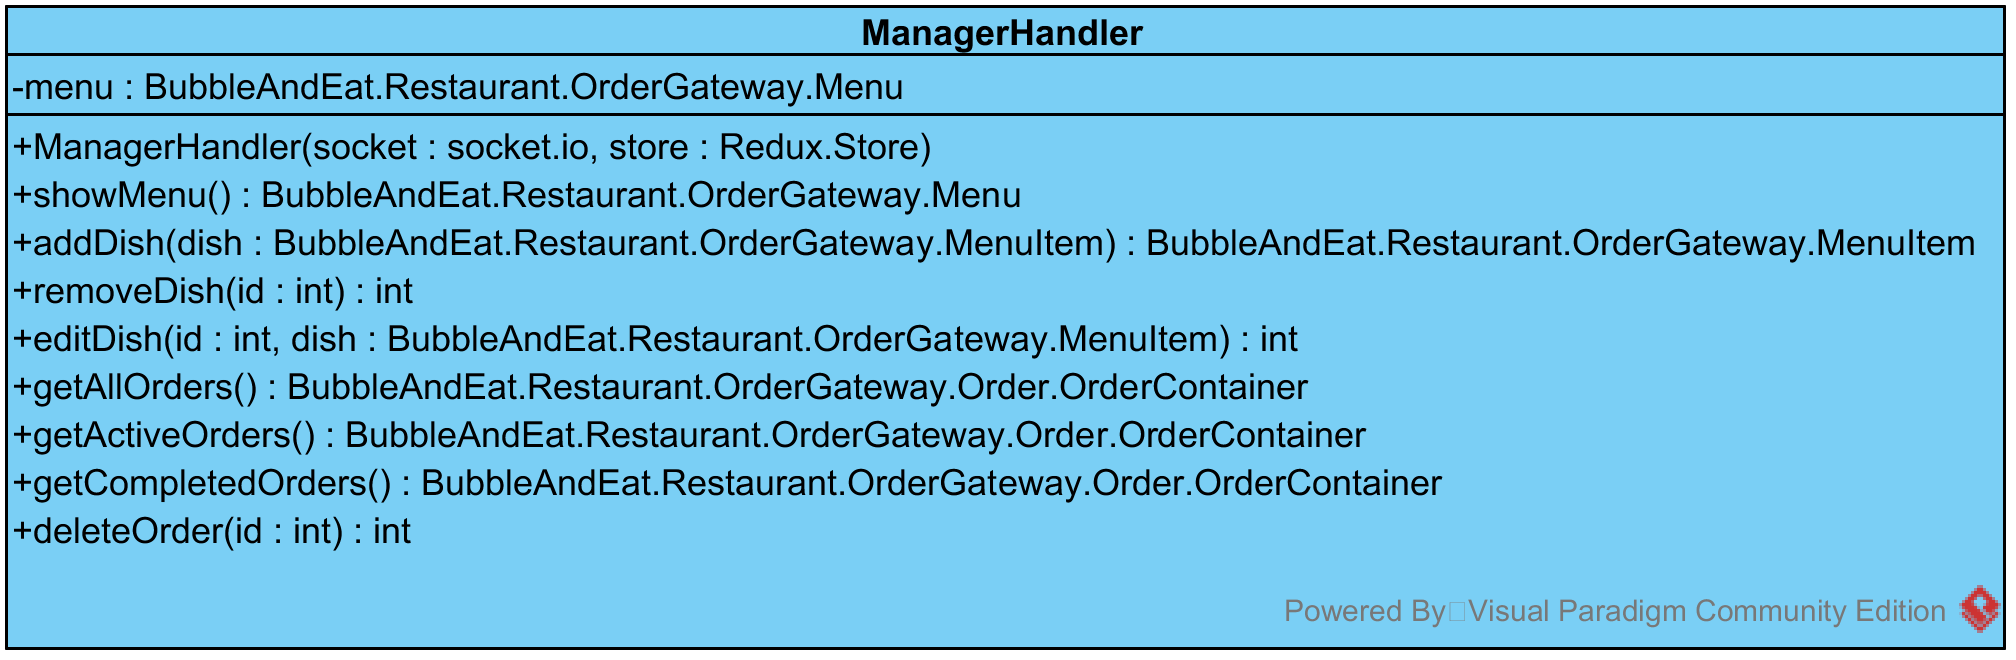
\includegraphics[width=15cm]{./diagrammi/demo/server/handlers/managerhandler.png}
	\caption{Classe \class}
\end{figure}
\textbf{Descrizione:}\\
Classe che gestisce le richieste provenienti dalla bubble ManagerBubble.

\textbf{Utilizzo:}\\
Viene utilizzata per gestire l'autenticazione del Manager ed eseguire le operazioni richieste dalla bubble lato client sul server.

\textbf{Classi ereditate:}
\begin{itemize}
	\item \coderef{BubbleAndEat::Restaurant::OrderGateway::Handlers::Handler}.
\end{itemize}
%
%\textbf{Sottoclassi:}
%\begin{itemize}
%	\item \coderef{}.
%\end{itemize}

\textbf{Attributi:}
\begin{itemize}
	\item \field{- menu: Menu}: menu del ristorante.
\end{itemize}

\textbf{Metodi:}
\begin{itemize}
	\item \method{+ ManagerHandler(socket: socket.io, store: Redux::Store)}: costruttore, assegna i parametri agli attributi:
	\begin{itemize}
		\item \param{socket: socket.io}: socket contenente i parametri di connessione;
		\item \param{store: Redux::Store}: store dell'applicazione;
	\end{itemize}
	\item \method{+ showMenu(): Menu}: ritorna il menu del ristorante;
	\item \method{+ addDish(dish: MenuItem): MenuItem}: aggiunge una pietanza al menu:
	\begin{itemize}
		\item \param{dish: MenuItem}: la pietanza da aggiungere;
	\end{itemize}
	\item \method{+ removeDish(id: int): int}: rimuove la pietanza dal menu:
	\begin{itemize}
		\item \param{id: int}: id della pietanza da rimuovere;
	\end{itemize}
	\item \method{+ editDish(id: int, dish: MenuItem): MenuItem}: modifica la pietanza del menu in \texttt{dish}:
	\begin{itemize}
		\item \param{id: int}: id della pietanza da modificare;
		\item \param{dish: MenuItem}: pietanza con dati aggiornati;
	\end{itemize}
	\item \method{+ getAllOrders(): OrderContainer}: ritorna tutti gli ordini presenti nell'applicazione;
	\item \method{+ getActiverOrders(): OrderContainer}: ritorna tutti gli ordini attivi (non completati) dell'applicazione;
	\item \method{+ getCompletedOrders(): OrderContainer}: ritorna tutti gli ordini completati dell'applicazione;
	\item \method{+ deleteOrder(id: int): int}: elimina l'ordine dall'applicazione:
	\begin{itemize}
		\item \param{id: int}: id dell'ordine da eliminare.
	\end{itemize}
\end{itemize}

\setclass{BubbleAndEat::Restaurant::OrderGateway::Handlers::ChefHandler}
\subparagraph[::ChefHandler]{\class}\mbox{}\\ \label{\class}
\begin{figure}[H]
	\centering
		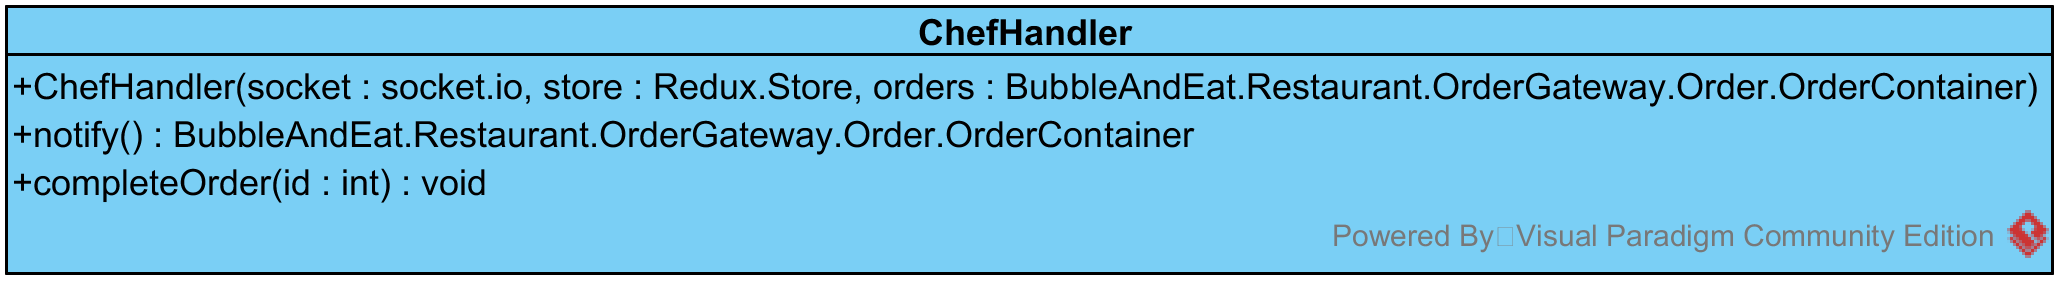
\includegraphics[width=15cm]{./diagrammi/demo/server/handlers/chefhandler.png}
	\caption{Classe \class}
\end{figure}
\textbf{Descrizione:}\\
Classe che gestisce le richieste provenienti dalla bubble ChefBubble.

\textbf{Utilizzo:}\\
Viene utilizzata per gestire l'autenticazione dello Chef ed eseguire le operazioni richieste dalla bubble lato client sul server.

\textbf{Classi ereditate:}
\begin{itemize}
	\item \coderef{BubbleAndEat::OrderGateway::Handlers::Handler}.
\end{itemize}
%
%\textbf{Sottoclassi:}
%\begin{itemize}
%	\item \coderef{}.
%\end{itemize}

%\textbf{Attributi:}
%\begin{itemize}
%\end{itemize}

\textbf{Metodi:}
\begin{itemize}
	\item \method{+ ChefHandler(socket: socket.io, store: Redux::Store, orders: OrderContainer)}: costruttore, assegna i parametri agli attributi e salva nello store la presenza dello Chef:
	\begin{itemize}
		\item \param{socket: socket.io}: socket contenente i parametri di connessione;
		\item \param{store: Redux::Store}: store dell'applicazione;
		\item \param{orders: OrderContainer}: contenitore di ordini nello stato di \virgolette{attivo};
	\end{itemize}
	\item \method{+ notify(): OrderContainer}: notifica lo Chef di una nuova ordinazione da preparare;
	\item \method{+ completeOrder(id: int): void}: salva l'ordine come completato:
	\begin{itemize}
		\item \param{id: int}: id dell'ordine completato.
	\end{itemize}
\end{itemize}


\setclass{BubbleAndEat::Restaurant::OrderGateway::Handlers::CustomerHandler}
\subparagraph[::CustomerHandler]{\class}\mbox{}\\ \label{\class}
\begin{figure}[H]
	\centering
		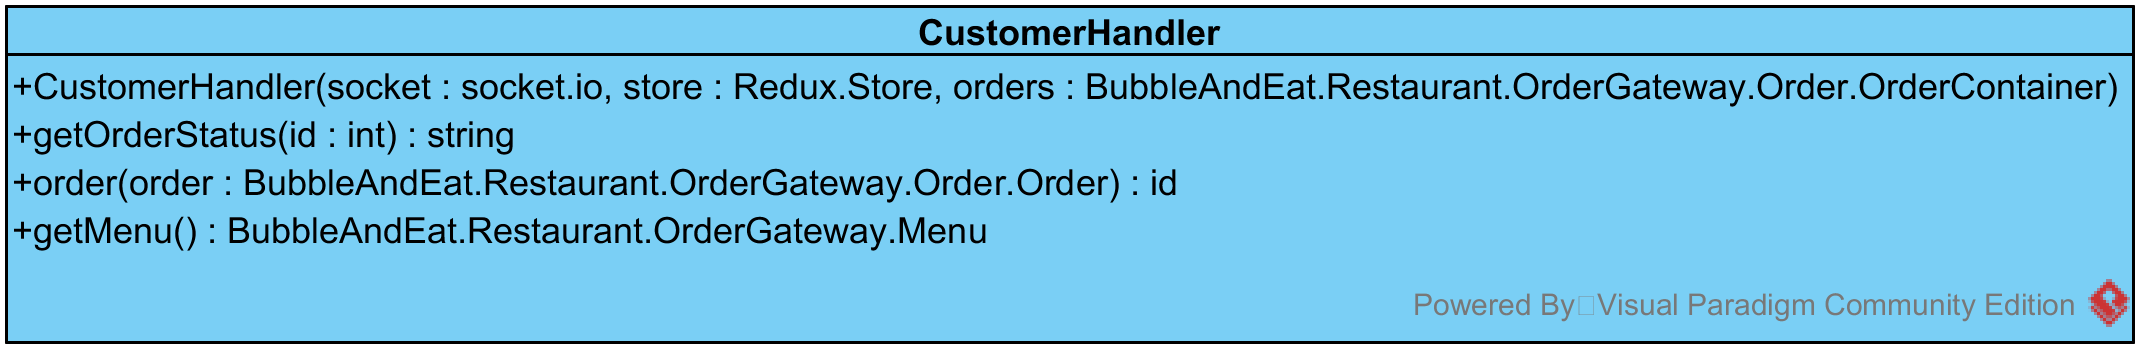
\includegraphics[width=15cm]{./diagrammi/demo/server/handlers/customerhandler.png}
	\caption{Classe \class}
\end{figure}
\textbf{Descrizione:}\\
Classe che gestisce le richieste provenienti dalla bubble CustomerBubble.

\textbf{Utilizzo:}\\
Viene utilizzata per gestire l'autenticazione del Customer ed eseguire le operazioni richieste dalla bubble lato client sul server.

\textbf{Classi ereditate:}
\begin{itemize}
	\item \coderef{BubbleAndEat::Restaurant::OrderGateway::Handlers::Handler}.
\end{itemize}
%
%\textbf{Sottoclassi:}
%\begin{itemize}
%	\item \coderef{}.
%\end{itemize}

%\textbf{Attributi:}
%\begin{itemize}
%\end{itemize}

\textbf{Metodi:}
\begin{itemize}
	\item \method{+ CustomerHandler(socket: socket.io, store: Redux::Store, orders: OrderContainer)}: costruttore, assegna i parametri agli attributi:
	\begin{itemize}
		\item \param{socket: socket.io}: socket contenente i parametri di connessione;
		\item \param{store: Redux::Store}: store dell'applicazione;
		\item \param{orders: OrderContainer}: ordini effettuati dal cliente;
	\end{itemize}
	\item \method{+ getOrderStatus(id: int): string}: ritorna lo stato dell'ordine:
	\begin{itemize}
		\item \param{id: int}: id dell'ordine di cui si vuole conoscere lo stato;
	\end{itemize}
	\item \method{+ order(order: Order): id}: processa l'ordine confermato dal Customer e gli assegna un id, che viene ritornato al Customer cosicché egli possa tracciare lo stato dell'ordine stesso:
	\begin{itemize}
		\item \param{order: Order}: l'ordine confermato e inviato;
	\end{itemize}
	\item \method{+ getMenu(): Menu}: recupera il menu dallo store e lo ritorna.
\end{itemize}

\setclass{BubbleAndEat::Restaurant::OrderGateway::MenuItem}
\paragraph[::MenuItem]{\class}\mbox{}\\ \label{\class}
\begin{figure}[H]
	\centering
	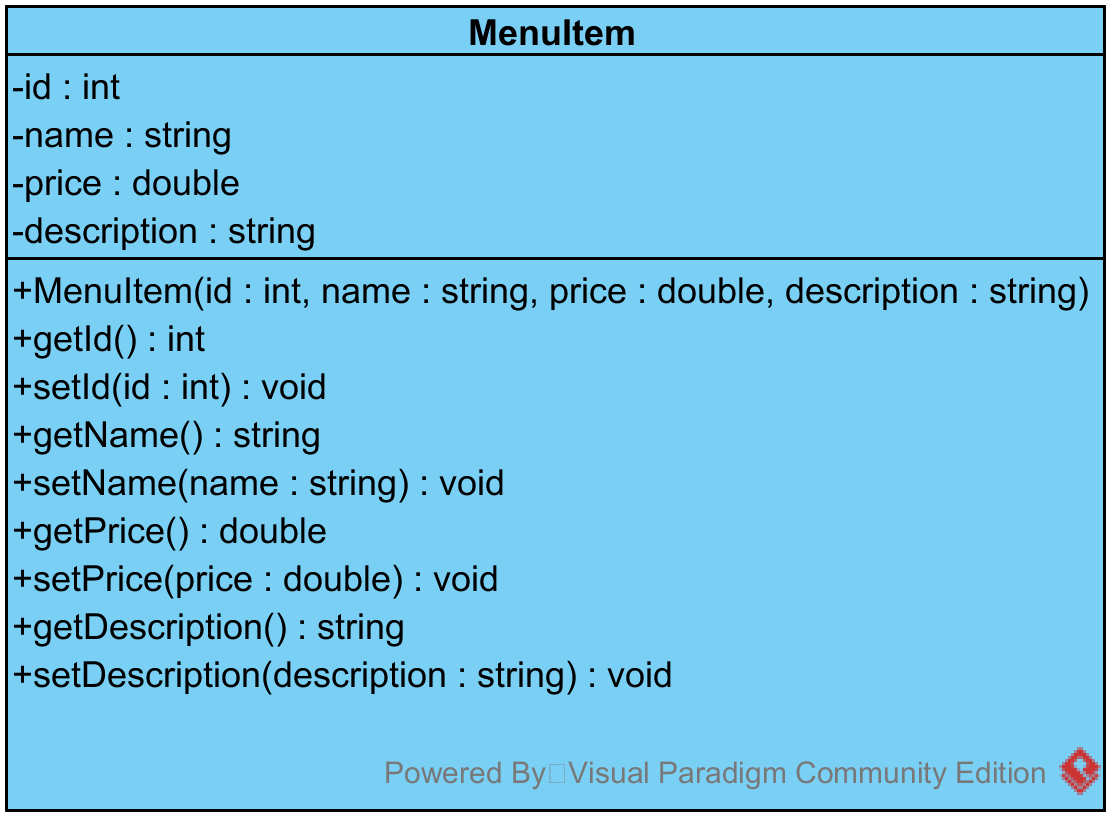
\includegraphics[width=10cm]{./diagrammi/demo/server/menuitem.png}
	\caption{Classe \class}
\end{figure}
\textbf{Descrizione:}\\
Classe che rappresenta una singola voce del menu.

\textbf{Utilizzo:}\\
Viene utilizzata per creare le singole pietanze da mostrare nel menu e da inserire negli ordini.

%\textbf{Classi ereditate:}
%\begin{itemize}
%	\item \code{}.
%\end{itemize}
%
%\textbf{Sottoclassi:}
%\begin{itemize}
%	\item \coderef{}.
%\end{itemize}

\textbf{Attributi:}
\begin{itemize}
	\item \field{- id: int}: numero identificativo della pietanza del menu;
	\item \field{- name: string}: nome della pietanza;
	\item \field{- price: double}: prezzo della pietanza;
	\item \field{- description: string}: descrizione della pietanza.
\end{itemize}

\textbf{Metodi:}
\begin{itemize}
	\item \method{+ MenuItem(id: int, name: string, price: double, description: string)}: costruttore, assegna i parametri ai corrispondenti attributi:
	\begin{itemize}
		\item \param{id: int}: id della pietanza;
		\item \param{name: string}: nome della pietanza;
		\item \param{price: double}: prezzo della pietanza;
		\item \param{description: string}: descrizione della pietanza;
	\end{itemize}
	\item \method{+ getId(): int} getter per \texttt{id};
	\item \method{+ setId(id: int): void}: setter per \texttt{id};
	\item \method{+ getName(): string} getter per \texttt{name};
	\item \method{+ setName(name: string): void}: setter per \texttt{name};
	\item \method{+ getPrice(): double} getter per \texttt{price};
	\item \method{+ setPrice(price: double): void}: setter per \texttt{price};
	\item \method{+ getDescription(): string} getter per \texttt{description};
	\item \method{+ setDesctiption(description: string): void}: setter per \texttt{description};
\end{itemize}

\setclass{BubbleAndEat::Restaurant::OrderGateway::Menu}
\paragraph[::Menu]{\class}\mbox{}\\ \label{\class}
\begin{figure}[H]
	\centering
	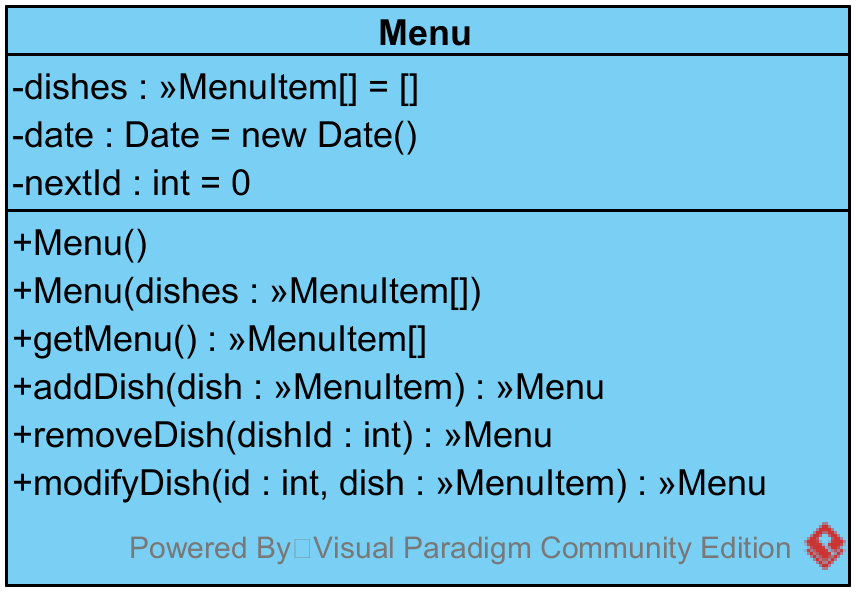
\includegraphics[width=8cm]{./diagrammi/demo/server/menu.png}
	\caption{Classe \class}
\end{figure}
\textbf{Descrizione:}\\
Classe che rappresenta il menu.

\textbf{Utilizzo:}\\
Viene utilizzata per raccogliere e gestire le pietanze disponibili nel ristorante.

%\textbf{Classi ereditate:}
%\begin{itemize}
%	\item \code{}.
%\end{itemize}
%
%\textbf{Sottoclassi:}
%\begin{itemize}
%	\item \coderef{}.
%\end{itemize}

\textbf{Attributi:}
\begin{itemize}
	\item \field{- dishes: MenuItem[] = []}: array contenete le pietanze del menu;
	\item \field{- date: Date = new Date()}: data di creazione del menu;
	\item \field{- nextId: int = 0}: numero di pietanze inserite e id per la nuova pietanza da inserire.
\end{itemize}

\textbf{Metodi:}
\begin{itemize}
	\item \method{+ Menu()}: costruttore di default;
	\item \method{+ Menu(dishes: MenuItem[])}: costruttore, inizializza l'array delle pietanze:
	\begin{itemize}
		\item \param{dishes: MenuItem[]}: array di pietanze;
	\end{itemize}
	\item \method{+ getMenu(): MenuItem[]} getter per \texttt{dishes};
	\item \method{+ addDish(dish: MenuItem): Menu}: permette di aggiungere una pietanza al menu:
	\begin{itemize}
		\item \param{dish: Menuitem}: pietanza da aggiungere
	\end{itemize}
	\item \method{+ removeDish(dishId: int): Menu} rimuove la pietanza con id \texttt{dishId} dal menu:
	\begin{itemize}
		\item \param{dishId: int}: id della pietanza da rimuovere;
	\end{itemize}
	\item \method{+ modifyDish(id: int, dish: MenuItem): Menu}: modifica la pietanza con id \texttt{id} in \texttt{dish}:
	\begin{itemize}
		\item \param{id: int}: id della pietanza da modificare;
		\item \param{dish: MenuItem}: pietanza con informazioni aggiornate.
	\end{itemize}
\end{itemize}

\setclass{BubbleAndEat::Restaurant::OrderGateway::Order}
\paragraph[::Order]{\class}\mbox{}\\ \label{\class}
\begin{figure}[H]
	\centering
	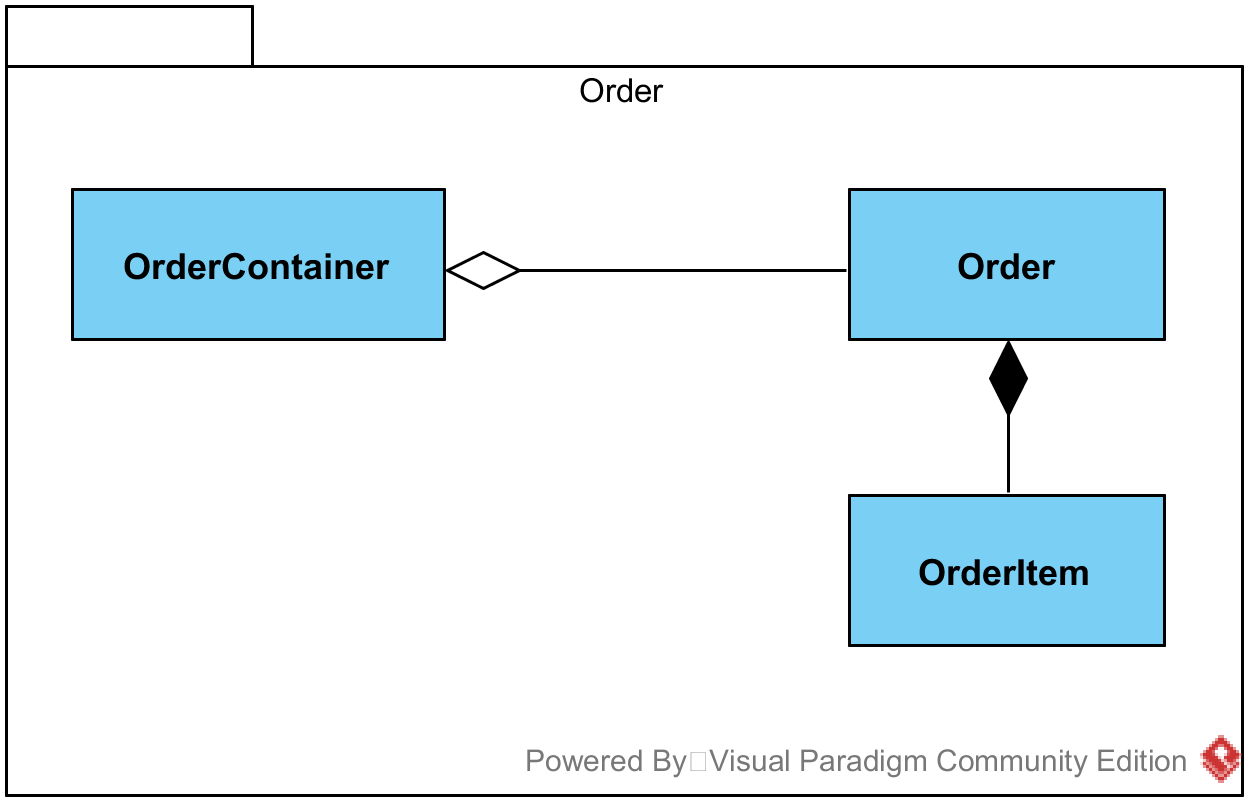
\includegraphics[width=12cm]{./diagrammi/demo/server/orderpkg.png}
	\caption{Componente \class}
\end{figure}

Questo componente ha la funzione di rappresentare gli ordini.

\setclass{BubbleAndEat::Restaurant::OrderGateway::Order::OrderContainer}
\subparagraph[::OrderContainer]{\class}\mbox{}\\ \label{\class}
\begin{figure}[H]
	\centering
	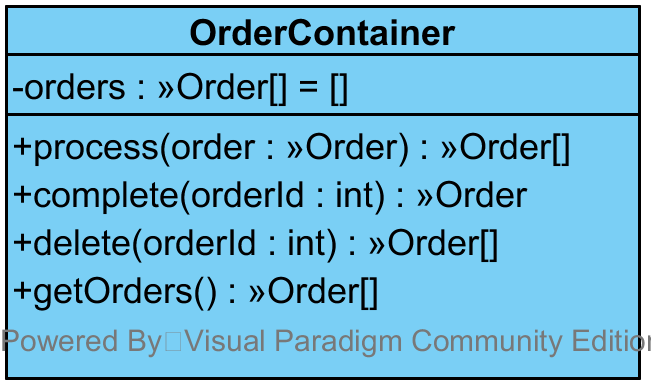
\includegraphics[width=7cm]{./diagrammi/demo/server/order/ordercontainer.png}
	\caption{Classe \class}
\end{figure}
\textbf{Descrizione:}\\
Classe che rappresenta un contenitore per gli ordini.

\textbf{Utilizzo:}\\
Viene utilizzata come contenitore comune degli ordini attivi per tutti gli utenti interni al ristorante.

%\textbf{Classi ereditate:}
%\begin{itemize}
%	\item \code{}.
%\end{itemize}
%
%\textbf{Sottoclassi:}
%\begin{itemize}
%	\item \coderef{}.
%\end{itemize}

\textbf{Attributi:}
\begin{itemize}
	\item \field{- {orders: Order[] = []}}: array contenente gli ordini, inizializzato di default ad un array vuoto.
\end{itemize}

\textbf{Metodi:}
\begin{itemize}
	\item \method{+ process(order: Order): Order[]}: processa l'ordine, lo imposta come attivo e lo aggiunge all'array \texttt{orders}:
	\begin{itemize}
		\item \param{order: Order}: il nuovo ordine da processare;
	\end{itemize}
	\item \method{+ complete(orderId: int): Order}: l'ordine con id \texttt{orderId} viene completato e il suo stato aggiornato;
	\item \method{+ delete(orderId: int): Order[]}: l'ordine con id \texttt{orderId} viene eliminato dalla lista degli ordini attivi;
	\item \method{+ getOrders(): Order[]}: getter per \texttt{orders}.
\end{itemize}

\setclass{BubbleAndEat::Restaurant::OrderGateway::Order::Order}
\subparagraph[::Order]{\class}\mbox{}\\ \label{\class}
\begin{figure}[H]
	\centering
	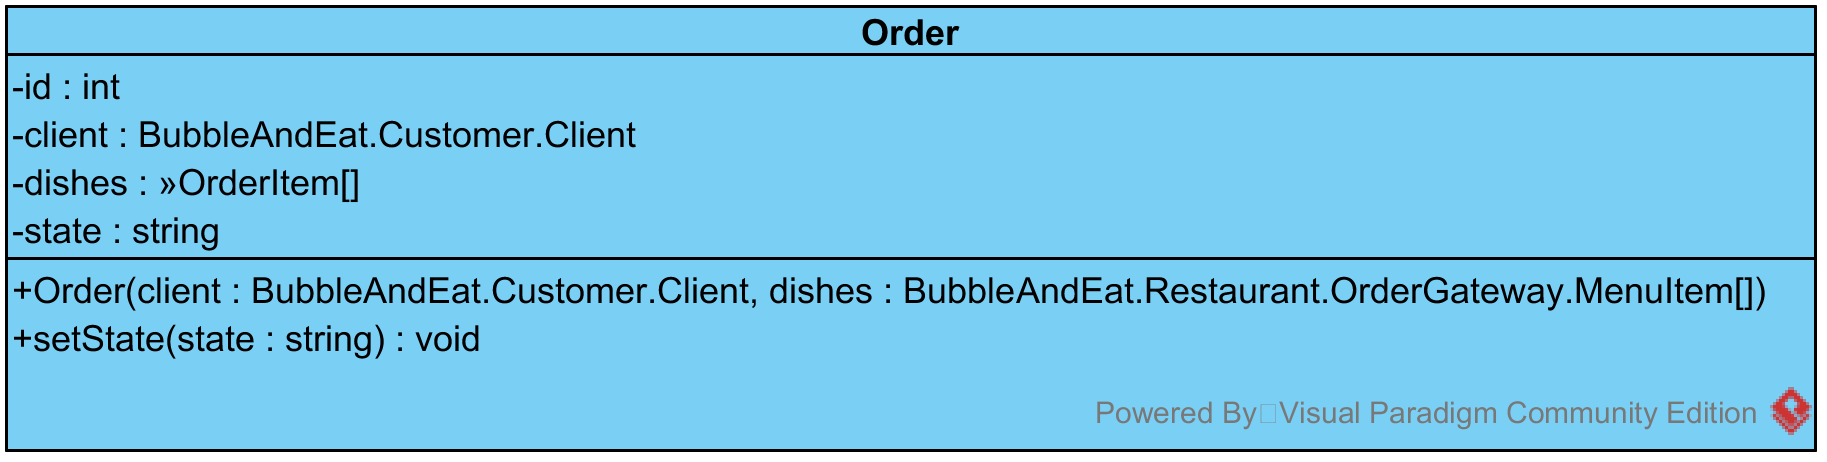
\includegraphics[width=12cm]{./diagrammi/demo/server/order/order.png}
	\caption{Classe \class}
\end{figure}
\textbf{Descrizione:}\\
Classe che rappresenta un singolo ordine.

\textbf{Utilizzo:}\\
Viene utilizzata per rappresentare i singoli ordini effettuati dai clienti, ovvero l'insieme delle pietanze che un utente ha ordinato.

%\textbf{Classi ereditate:}
%\begin{itemize}
%	\item \code{}.
%\end{itemize}
%
%\textbf{Sottoclassi:}
%\begin{itemize}
%	\item \coderef{}.
%\end{itemize}

\textbf{Attributi:}
\begin{itemize}
	\item \field{- id: int}: numero identificativo dell'ordine;
	\item \field{- client: Client}: cliente che ha effettuato l'ordine;
	\item \field{- dishes: OrderItem[]}: lista dei piatti ordinati;
	\item \field{- state: string}: indica lo stato di avanzamento dell'ordine.
\end{itemize}

\textbf{Metodi:}
\begin{itemize}
	\item \method{+ Order(client: Client, dishes: OrderItem[])}: costruttore, crea un nuovo ordine con cliente e pietanze ordinate:
	\begin{itemize}
		\item \param{client: Client}: cliente che ha effettuato l'ordine;
		\item \param{dishes: MenuItem[]}: pietanze ordinate;
	\end{itemize}
	\item \method{+ setState(state: string): void}: permette di aggiornare lo stato dell'ordine.
\end{itemize}

\setclass{BubbleAndEat::Restaurant::OrderGateway::OrderItem}
\subparagraph[::OrderItem]{\class}\mbox{}\\ \label{\class}
\begin{figure}[H]
	\centering
	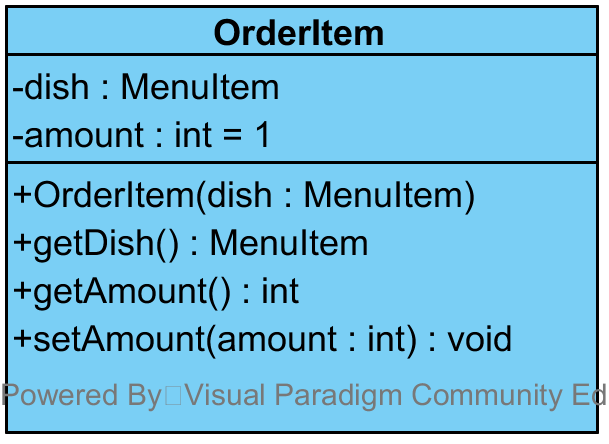
\includegraphics[width=12cm]{./diagrammi/demo/server/order/orderitem.png}
	\caption{Classe \class}
\end{figure}
\textbf{Descrizione:}\\
Classe che rappresenta una pietanza dell'ordine.

\textbf{Utilizzo:}\\
Viene utilizzata per memorizzare le quantità per ogni singolo piatto incluso nell'ordine.

%\textbf{Classi ereditate:}
%\begin{itemize}
%	\item \code{}.
%\end{itemize}
%
%\textbf{Sottoclassi:}
%\begin{itemize}
%	\item \coderef{}.
%\end{itemize}

\textbf{Attributi:}
\begin{itemize}
	\item \field{- dish: MenuItem}: piatto selezionato dal menu;
	\item \field{- amount: int = 1}: quantità selezionata (di default vale 1, altrimenti la voce dell'ordine non ha senso di esistere).
\end{itemize}

\textbf{Metodi:}
\begin{itemize}
	\item \method{+ OrderItem(dish: MenuItem)}: costruttore della classe, crea una voce dell'ordine per la pietanza \emph{dish};
	\item \method{+ getDish(): MenuItem}: getter per \texttt{dish};
	\item \method{+ getAmount(): int}: getter per \texttt{amount};
	\item \method{+ setAmount(amount: int): void}: setter per \texttt{amount}.
\end{itemize}